% ============================================================================
%  BLOQUE II — DIAPOSITIVAS 4–6: PROBLEMA Y OBJETIVOS
% ============================================================================
\section{Problema y Objetivos}

% ----------------------------------------------------------------------------
%  DIAPOSITIVA 4 — PROBLEMA + OBJETIVO GENERAL (fusionada)
% ----------------------------------------------------------------------------
\begin{frame}{Problema y Objetivo General}
  \hypertarget{s:problema}{}
  \begin{columns}[T]
    \column{0.5\textwidth}
    \begin{alertblock}{El problema}
      \footnotesize
      La domótica actual depende de servicios cloud: sin Internet,
      el hogar inteligente se vuelve inerte. Los datos de comportamiento
      viajan a servidores de terceros.
    \end{alertblock}

    \begin{exampleblock}{La respuesta}
      \footnotesize
      Sistema 100\% local de control de confort térmico orquestado
      por IA en el \textit{edge}. Interoperabilidad real sin modificar hardware.
    \end{exampleblock}

    \column{0.5\textwidth}
    \begin{block}{Objetivo general}
      \centering
      Diseñar, implementar y validar un sistema de monitorización
      y control de confort térmico que opere de forma autónoma
      en una red local privada, eliminando cualquier dependencia
      de servicios en la nube.
    \end{block}
  \end{columns}

  \vspace{0.4cm}
  \begin{columns}[T]
    \column{0.33\textwidth}
    \centering
    \textcolor{primary}{\textbf{Coste cero}}\\[0.1cm]
    {\footnotesize 0 € en licencias, APIs externas o suscripciones}
    \column{0.33\textwidth}
    \centering
    \textcolor{primary}{\textbf{Reproducibilidad}}\\[0.1cm]
    {\footnotesize Mismo hardware $\rightarrow$ replicar con la documentación}
    \column{0.33\textwidth}
    \centering
    \textcolor{primary}{\textbf{Hardware real}}\\[0.1cm]
    {\footnotesize Pruebas sobre dispositivos físicos, no simulación}
  \end{columns}
\end{frame}

% ----------------------------------------------------------------------------
%  DIAPOSITIVA 6 — OBJETIVOS ESPECÍFICOS E INDICADORES
% ----------------------------------------------------------------------------
\begin{frame}{Objetivos Específicos e Indicadores}
  \hypertarget{s:objetivos}{}
  \centering
  \IfFileExists{figures/08_objetivos.pdf}{%
    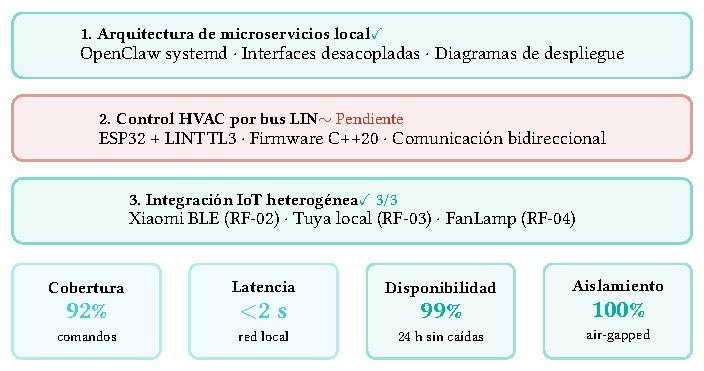
\includegraphics[width=0.92\textwidth, height=5.5cm, keepaspectratio]{figures/08_objetivos.pdf}%
  }{
    \textcolor{darkgray}{[Figura: dashboard de objetivos]}
  }
\end{frame}
